\documentclass[12pt, a4paper]{article}
\usepackage[utf8]{inputenc}
\usepackage[spanish]{babel}
\usepackage{enumitem}
\usepackage{url, hyperref}
\usepackage{listings, xcolor}
\usepackage{graphicx, subcaption}

\definecolor{codegreen}{rgb}{0,0.6,0}
\definecolor{codegray}{rgb}{0.5,0.5,0.5}
\definecolor{codepurple}{rgb}{0.58,0,0.82}
\definecolor{backcolour}{rgb}{0.95,0.95,0.92}
\lstdefinestyle{mystyle}{
    backgroundcolor=\color{backcolour},   
    commentstyle=\color{codegreen},
    keywordstyle=\color{magenta},
    numberstyle=\tiny\color{codegray},
    stringstyle=\color{codepurple},
    basicstyle=\ttfamily\footnotesize,
    breakatwhitespace=false,         
    breaklines=true,                 
    captionpos=b,                    
    keepspaces=true,                 
    numbers=left,                    
    numbersep=5pt,                  
    showspaces=false,                
    showstringspaces=false,
    showtabs=false,                  
    tabsize=2
}
\lstset{style=mystyle, language=Python}

\setlength{\parindent}{0pt}
\setlength{\parskip}{2pt}

\title{\vspace{-3cm}Examen Parcial 1: Procesamiento de imágenes}
\author{
    Universidad Autónoma de San Luis Potosí\\
    Facultad de Ingeniería - Ing. en Sistemas Inteligentes\\
    \textbf{Materia:} Visión Computacional\\
    \textbf{Prof:} Dr. Cesar Augusto Puente Montejano\\
    \textbf{Autor:} Angel de Jesús Maldonado Juárez
}
\date{\textbf{Fecha de entrega:} lunes 26 de septiembre de 2022}

\begin{document}
\maketitle

\section{Planteamiento del Problema}\label{Planteamiento}
Con base en la imagen \ref{img:examen}, se deben realizar las siguientes operaciones:

\begin{enumerate}[label=\alph*)]
    \item Aplicar el filtro de \emph{Sobel} sobre la imagen original y guardarla en una nueva.
    \item Aplicar el filtro \emph{Morfológico } las veces necesarias con el objetivo de definir de la mejor manera el rostro de la persona que aparece en la imagen.
    \item Recortar la imagen de manera que obtenga una nueva imagen con solo el rostro de la persona, como se muestra en la Figura \ref{img:ejemplo-1}.
    \item Aplicar un filtro (cualquiera) a la imagen de manera que el rostro de la persona aparezca lo más nítido posible.
    \item Rotar la imagen de manera que el rostro no presente ningún grado de inclinación. (Figura \ref{img:ejemplo-2})
\end{enumerate}

\begin{figure}[!ht]
    \centering
    \begin{subfigure}{0.3\textwidth}
        \centering
        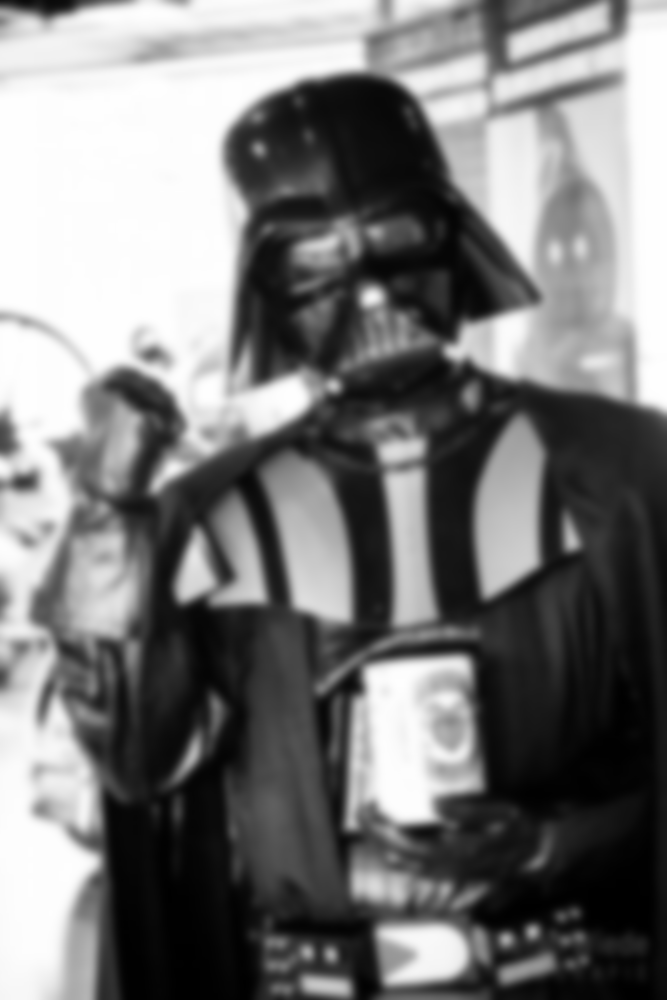
\includegraphics[width=0.5\textwidth]{img/examen_b.png}
        \caption{Imagen del examen}
        \label{img:examen}
    \end{subfigure}
    \hfill
    \begin{subfigure}{0.25\textwidth}
        \centering
        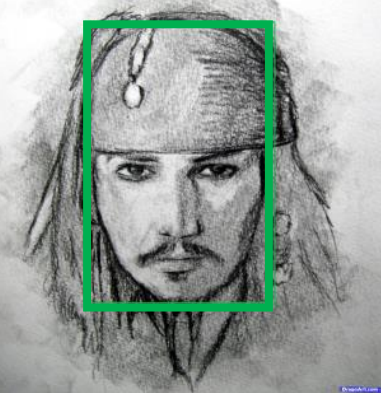
\includegraphics[width=0.85\textwidth]{img/sample-face-only.png}
        \caption{Ej. de recorte}
        \label{img:ejemplo-1}
    \end{subfigure}
    \hfill
    \begin{subfigure}{0.25\textwidth}
        \centering
        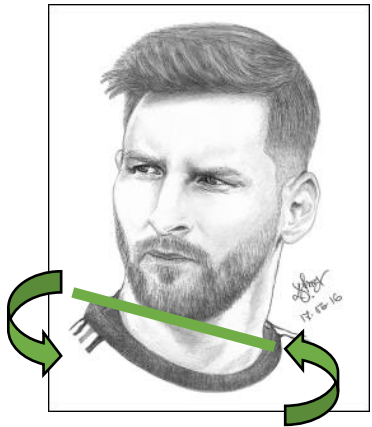
\includegraphics[width=0.8\textwidth]{img/sample-face-rotation.png}
        \caption{Ej. de rotación}
        \label{img:ejemplo-2}
    \end{subfigure}
    \caption{Imágenes del planteamiento}
\end{figure}

\section{Descripción de la Solución}
El programa escrito en \emph{Python} está hecho de forma que se pueda manipular la imagen de estudio en \textbf{tiempo real} y siguiendo la secuencia de pasos descrita en el \hyperref[Planteamiento]{Planteamiento del Problema}

En la parte superior del programa se definen y declaran los parámetros de los distintos filtros y otras operaciones que se van a aplicar:

\begin{lstlisting}
# Sobel filter parameters
dx_sobel = 1
dy_sobel = 0
ksize_sobel = 1

# Dilate initial parameters
shape_dilate = cv.MORPH_RECT
ksize_dilate = 1

# Erode filter parameters
shape_erode = cv.MORPH_RECT
ksize_erode = 1

# Rotation degrees
deg = 0

# Crop coordinates
point_matrix = np.zeros((2, 2), np.int32)
# Click counter
click_counter = 0
\end{lstlisting}

Después de cargar la imagen con la función \lstinline{cv.imread()} y de verificar que se cargó correctamente con \lstinline{img.size != 0}, se crea la ventana principal con \lstinline{cv.namedWindow()}, e inicia el primer ciclo para aplicar el \emph{filtro Sobel}. Todos los ciclos del programa tienen la misma estructura:

\begin{lstlisting}
while True:
    # Principal operation

    # Show current parameters on console

    # Show image with applied operation

    # Wait for user key and manage it
\end{lstlisting}

En la etapa en la que se espera por la entrada/tecla del usuario, se definen para todos los ciclos del programa que la tecla 'x' es para cerrar el programa, y la tecla 'Enter' es para avanzar al siguiente paso.

Finalmente, después de haber aplicado todos los filtros y operaciones que se plantean, se muestra un último mensaje en consola con los parámetros de todos los filtros y operaciones finales:

\begin{lstlisting}
print('\nSobel parameters: dx={}, dy={}, ksize={}'.format(
    dx_sobel, dy_sobel, ksize_sobel))
print("Dilate parameters: shape={}, ksize={}".format(
    str(shape_dilate), ksize_dilate))
print("Crop coordinates: ({},{}) ({},{})".format(
    point_matrix[0][0], point_matrix[0][1], point_matrix[1][0], point_matrix[1][1]))
print("Erode parameters: shape={}, ksize={}".format(
    str(shape_erode), ksize_erode))
print("Rotating angle: {}".format(deg))
\end{lstlisting}

\section{Descripción de los Resultados}
\textbf{Filtro Sobel}

OpenCV permitía dejar en $0$ los valores \emph{deltas} de $x$ y $y$, sin embargo, el mejor resultado se logró con ambos parámetros activos. Con estos valores se pueden distinguir muy bien los bordes de las figuras de la imagen.

\textbf{Filtro Dilate}

Con este filtro se espera subir considerablemente las regiones con brillo de la imagen, y ya que el objetivo es identificar el rostro (casco), es ideal llegar a un punto preciso de brillo en el que el contorno del casco quede bien delimitado por regiones con brillo.

\textbf{Filtro Erode}

Este filtro fue la mejor elección, ya que contrarresta al anterior para poder dejar las regiones bien delimitadas, con el suficiente brillo para que sean distinguibles, pero también con zonas oscuras para la suficiente profundidad a la imagen.

\begin{figure}[!ht]
    \centering
    \begin{subfigure}{0.23\textwidth}
        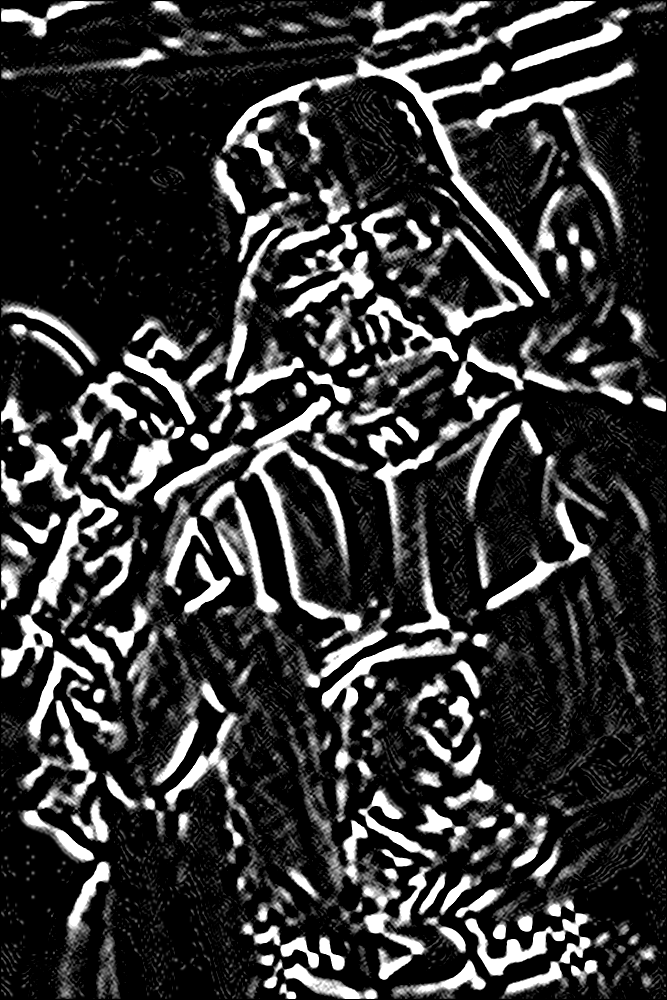
\includegraphics[width=\textwidth]{img/sobel-res.png}
        \caption{Filtro Sobel}
    \end{subfigure}
    \hfill
    \begin{subfigure}{0.23\textwidth}
        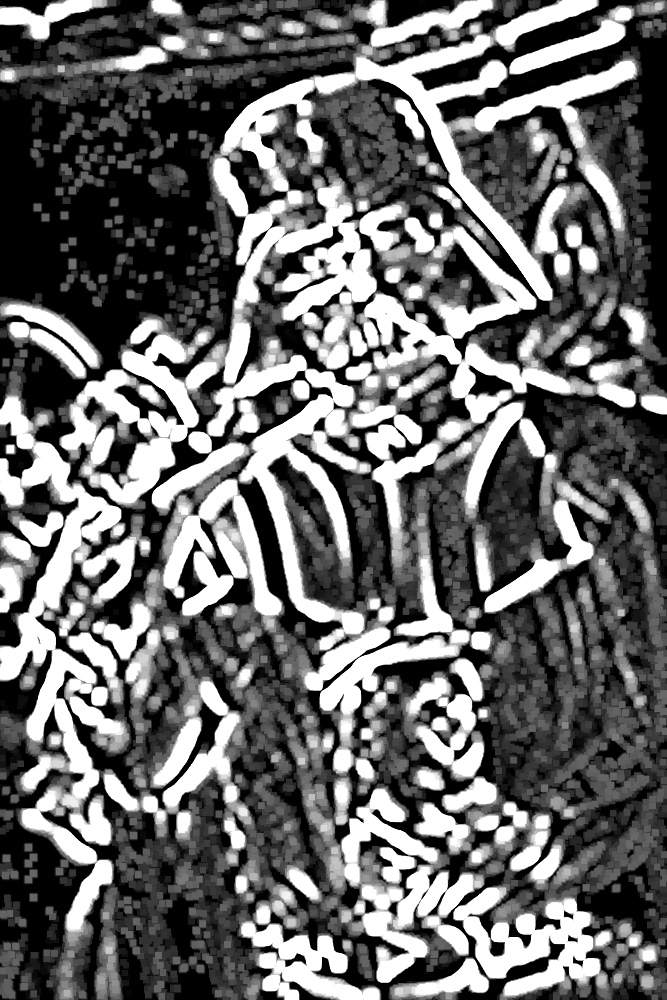
\includegraphics[width=\textwidth]{img/dilate-res.png}
        \caption{Filtro Dilate}
    \end{subfigure}
    \hfill
    \begin{subfigure}{0.3\textwidth}
        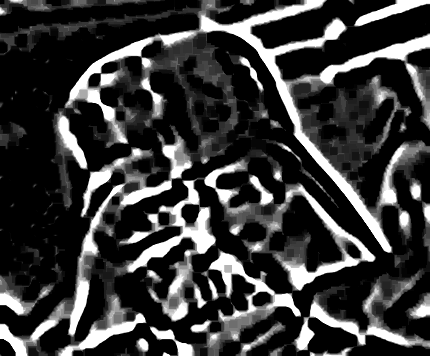
\includegraphics[width=\textwidth]{img/erode-res.png}
        \caption{Filtro Erode}
    \end{subfigure}
\end{figure}

Finalmente, la rotación de la última transformación para alinear el casco de forma horizontal logra dar la vista final y nítida del rostro del personaje \emph{Darth Vader}, junto con el recorte de la matriz de la imagen para enfocar solamente el casco:

\begin{figure}[!ht]
    \centering
    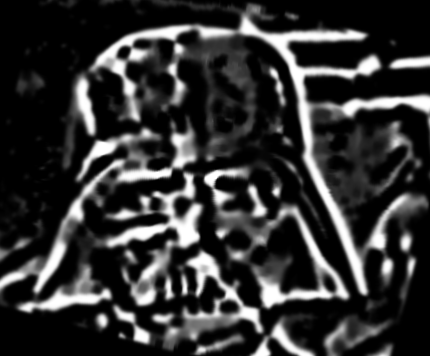
\includegraphics[width=0.5\textwidth]{img/res.png}
    \caption{Imagen final}
\end{figure}

Y mostrando en consola los parámetros utilizados en cada filtro y transformación de la imagen:

\begin{figure}[!ht]
    \centering
    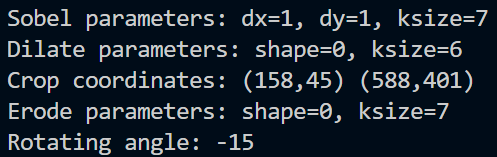
\includegraphics[width=0.9\textwidth]{img/res-parameters.png}
    \caption{Parámetros de operaciones con la imagen en consola}
\end{figure}

\section{Discusión}
En primera instancia los resultados llegaron a ser desconcertantes, debido a la abstracción de la imagen por el filtro Sobel. Sin embargo, conforme se fueron manipulando los parámetros de cada filtro, y repitiendo el proceso varias veces ahora se distingue y entiende finalmente la información de la imagen y el objetivo final.

\section{Conclusión}
El procesamiento de imágenes es un área sin duda de gran importancia en la Visión Computacional, e incluso en otros campos del conocimiento. Ya que el objetivo de las operaciones dentro del procesamiento de imágenes es mejorar la información de un mapa de bits de tal forma que el humano pueda ver mejor una imagen, o que una computadora la reconozca más fácil.

\bibliographystyle{plain}
\bibliography{refs}
\nocite{*}
\end{document}